\section{Kiến trúc tổng quan}

\begin{center}

\includegraphics[height=0.65\textheight,width=\textwidth,keepaspectratio]{img/mermaid/arch_overview.pdf}
\captionof{figure}{Kiến trúc tổng quan hệ thống Audit Log}
\label{fig:arch-overview}
\end{center}

Luồng xử lý: \texttt{app\_user} thực hiện \ac{dml} (INSERT/UPDATE/DELETE) trên các bảng nghiệp vụ $\rightarrow$ \textbf{AFTER ROW trigger} gọi \textbf{generic audit function} $\rightarrow$ ghi vào \texttt{audit\_logs} (partitioned) với dữ liệu \texttt{old\_data/new\_data} dạng JSONB $\rightarrow$ lớp bảo mật (append-only) và cơ chế cảnh báo (\texttt{security\_alerts}) có thể tích hợp Monitoring/SIEM.

\section{Thiết kế mô hình dữ liệu audit (Schema Design)}

Mục tiêu: ghi vết đầy đủ nhưng tối ưu cho hệ thống \textbf{write-heavy} theo yêu cầu ISO/IEC 27002:2022 \cite{ISO27002}.

\begin{center}
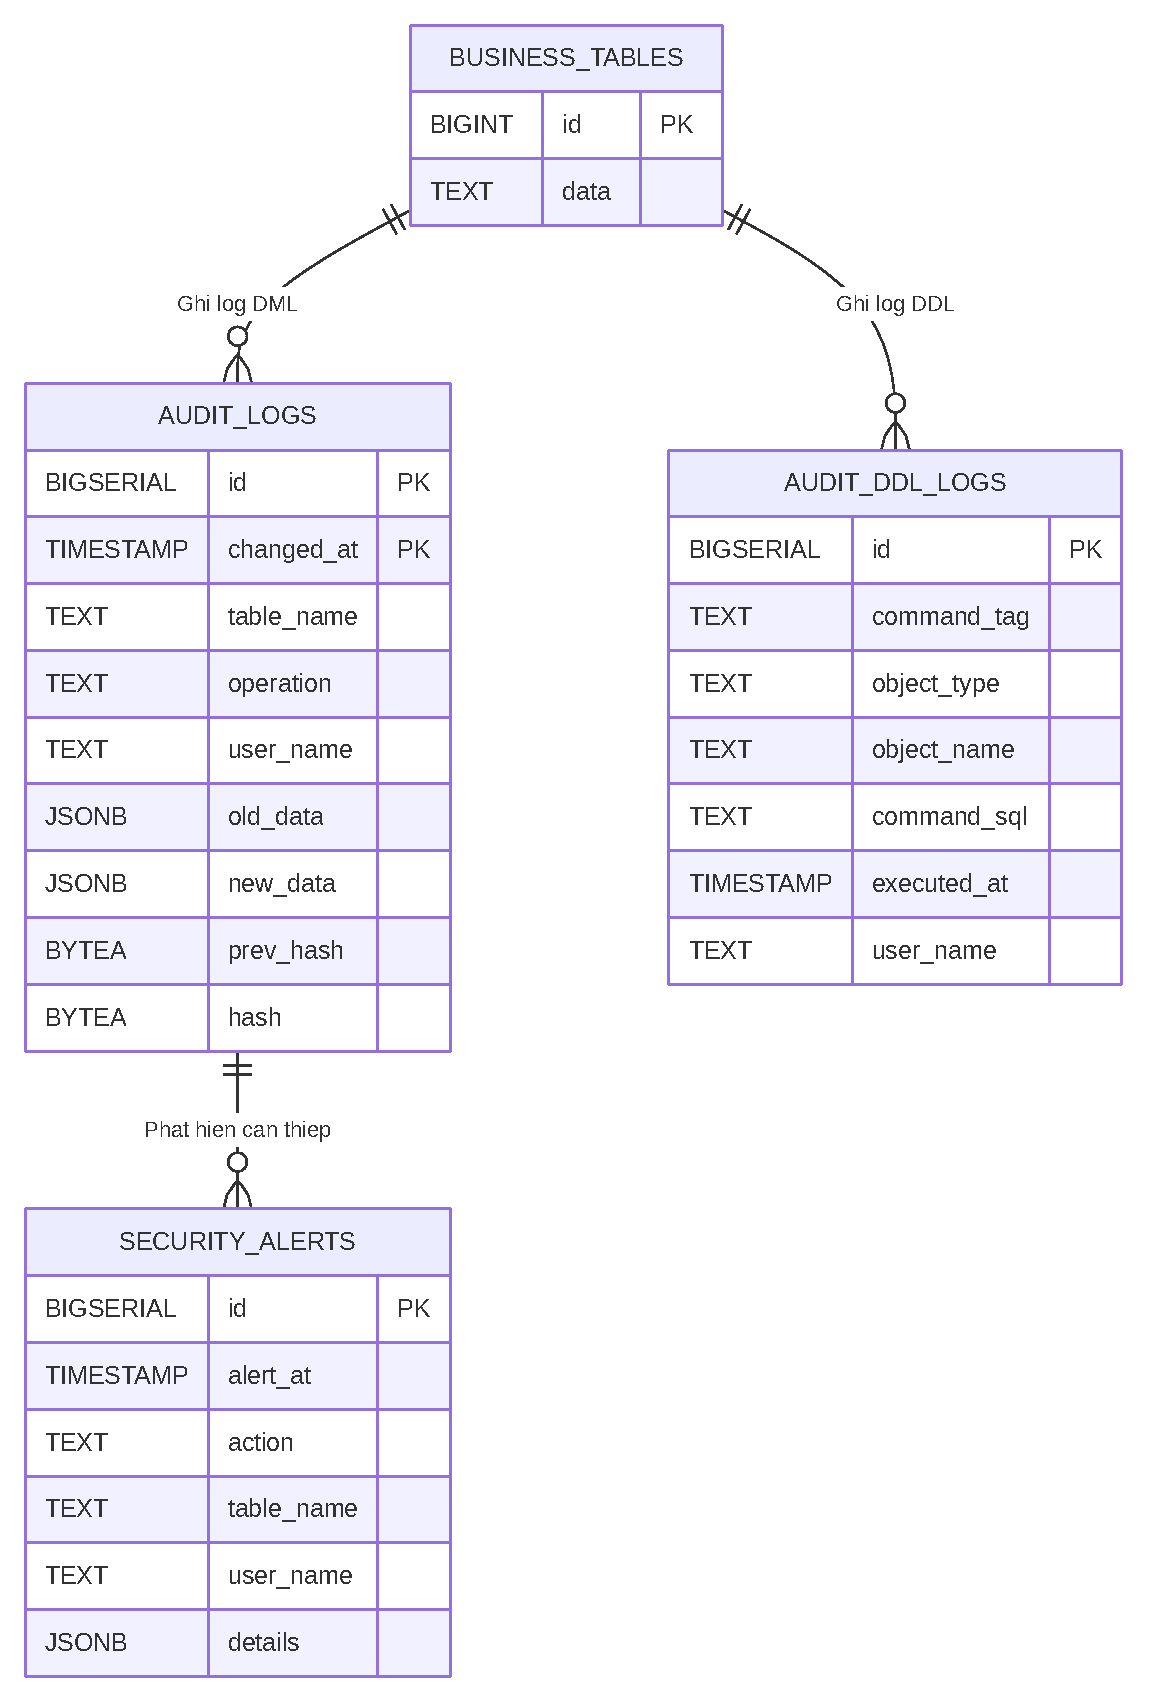
\includegraphics[width=\textwidth]{img/mermaid/er_diagram.pdf}
\captionof{figure}{Sơ đồ thực thể (ER) hệ thống Audit Log}
\label{fig:er-diagram}
\end{center}

\subsection{Bảng audit\_logs}

Bảng \texttt{audit\_logs} lưu trữ mọi thay đổi DML từ các bảng nghiệp vụ:

\begin{center}
\captionof{listing}{DDL bảng audit\_logs (partitioned JSONB)}
\label{lst:ddl-audit-logs}
\begin{Verbatim}[frame=single, fontsize=\footnotesize, numbers=left, numbersep=5pt, breaklines]
CREATE TABLE audit_logs (
    id          BIGSERIAL,
    table_name  TEXT      NOT NULL,
    operation   TEXT      NOT NULL,   -- INSERT / UPDATE / DELETE
    user_name   TEXT,
    old_data    JSONB,
    new_data    JSONB,
    changed_at  TIMESTAMP NOT NULL DEFAULT CURRENT_TIMESTAMP,
    prev_hash   BYTEA,                -- tamper-evident chain
    hash        BYTEA,
    PRIMARY KEY (id, changed_at)
) PARTITION BY RANGE (changed_at);
\end{Verbatim}
\end{center}

Nguyên tắc:
\begin{itemize}
    \item \textbf{Schema-less logging:} 1 bảng audit phục vụ nhiều bảng nghiệp vụ.
    \item \textbf{Append-only/WORM:} không cho UPDATE/DELETE log.
    \item Tối ưu truy vấn theo \textbf{thời gian} và theo \texttt{table\_name}/\texttt{actor}.
\end{itemize}

\begin{sloppypar}\noindent \textbf{Lưu ý quan trọng khi dùng Partitioning:} Partition key (\texttt{changed\_at}) phải nằm trong Primary Key của bảng cha (ví dụ: \texttt{(id, changed\_at)}), nếu không sẽ gặp ràng buộc/thiết kế không hợp lệ.\end{sloppypar}

\subsection{Bảng audit\_ddl\_logs}

Bảng này ghi lại mọi thay đổi schema (CREATE/ALTER/DROP) qua Event Trigger:

\begin{center}
\captionof{listing}{DDL bảng audit\_ddl\_logs}
\label{lst:ddl-audit-ddl-logs}
\begin{Verbatim}[frame=single, fontsize=\footnotesize, numbers=left, numbersep=5pt, breaklines]
CREATE TABLE public.audit_ddl_logs (
    id          BIGSERIAL PRIMARY KEY,
    command_tag TEXT      NOT NULL,   -- CREATE TABLE, ALTER TABLE, DROP TABLE, ...
    object_type TEXT,                 -- TABLE / INDEX / FUNCTION
    object_name TEXT,                 -- full object name within schema
    command_sql TEXT,                 -- command_tag || ' ' || object_identity
    executed_at TIMESTAMP NOT NULL DEFAULT CURRENT_TIMESTAMP,
    user_name   TEXT      NOT NULL DEFAULT session_user
);
\end{Verbatim}
\end{center}

Khác \texttt{audit\_logs}: không cần partitioning (tần suất ghi thấp hơn nhiều), không lưu JSONB old/new (DDL không có row-level data), dùng PK đơn giản (\texttt{BIGSERIAL}). Yêu cầu cài đặt bởi \textbf{superuser}.


\clearpage
\section{Thiết kế lưu trữ JSONB và lập chỉ mục}

JSONB là dạng JSON nhị phân đã parse \cite{PG16JSONB}, thuận lợi cho truy vấn có cấu trúc. Quy ước ghi dữ liệu:
\begin{itemize}
    \item \texttt{old\_data = to\_jsonb(OLD)}
    \item \texttt{new\_data = to\_jsonb(NEW)}
\end{itemize}

\textbf{Index strategy:}
\begin{itemize}
    \item \textbf{GIN index} \cite{PG16GIN} cho \texttt{new\_data}/\texttt{old\_data} để tìm kiếm theo key/value bên trong JSON.
    \item \begin{sloppypar}B-tree index cho (\texttt{changed\_at}), (\texttt{table\_name}, \texttt{changed\_at}), (\texttt{user\_name}, \texttt{changed\_at}).\end{sloppypar}
\end{itemize}

\section{Thiết kế Partitioning theo thời gian}

Declarative partitioning: \texttt{PARTITION\ BY\ RANGE\ (changed\_at)} \cite{PG16Partitioning} theo tháng.

\textbf{Lợi ích:}
\begin{itemize}
    \item \textbf{Partition pruning:} planner tự loại bỏ partition không liên quan khi truy vấn theo thời gian.
    \item Quản trị/retention đơn giản: drop partition thay vì delete từng dòng.
\end{itemize}

Tiêu chí kiểm soát archiving: chỉ \texttt{db\_admin} thực hiện; log thao tác archiving được ghi vào \texttt{audit\_ddl\_logs}; file dump được lưu trữ ít nhất 3 năm theo yêu cầu pháp lý.

\clearpage
\section{Phân tích đánh đổi (Trade-offs)}

\begin{center}
\centering
\captionof{table}{Phân tích đánh đổi thiết kế}
\label{tab:tradeoffs}
\renewcommand{\arraystretch}{1.4}
\begin{tabularx}{\textwidth}{>{\raggedright\arraybackslash}p{3.8cm}>{\raggedright\arraybackslash}X}
\toprule
\textbf{Quyết định} & \textbf{Phân tích} \\
\midrule
\textbf{JSONB} thay vì cột riêng &
  \textbf{(+)} 1 bảng audit cho nhiều table; không migration khi schema nghiệp vụ đổi \newline
  \textbf{($-$)} Storage +20--30\% so với typed columns; truy vấn phức tạp hơn; không thể dùng foreign key constraint \\
\textbf{Trigger} thay vì application logging &
  \textbf{(+)} Không cần sửa code app; log đảm bảo ngay cả khi app bypass \newline
  \textbf{($-$)} Overhead mỗi \ac{dml} (+1 INSERT); khó debug khi trigger lỗi; tăng WAL size \\
\textbf{Partitioning theo tháng} &
  \textbf{(+)} Partition pruning; DROP PARTITION O(1); tablespace tách biệt \newline
  \textbf{($-$)} Cross-partition query chậm hơn; PRIMARY KEY phải gồm partition key; tạo partition mới cần cron job \\
\textbf{Synchronous logging} &
  \textbf{(+)} Atomicity: log commit cùng transaction; không mất log khi crash \newline
  \textbf{($-$)} Không giảm được latency trigger; không phù hợp $>$10k TPS \\
\textbf{Hash chain SHA-256} &
  \textbf{(+)} Tamper-evident: phát hiện can thiệp ở tầng file; không thể phủ nhận \newline
  \textbf{($-$)} +1 SELECT prev\_hash mỗi INSERT; race condition khi concurrent writes \\
\bottomrule
\end{tabularx}
\renewcommand{\arraystretch}{1}
\end{center}
